\documentclass[a4paper,11pt]{scrartcl}
\usepackage[a4paper,left=1cm,right=2cm,top=2cm,bottom=4cm,bindingoffset=5mm]{geometry}
\usepackage[utf8]{inputenc}
\usepackage{tabularx}
\usepackage{multirow}
\usepackage{enumitem}
\usepackage{graphicx}


\begin{document}
	\centering \section*{Protokoll Resonanz}
	\begin{tabularx}{\textwidth}{r l r r}
			\multirow{2}{*}{Versuchsgruppe:}
				&Dercio Cipriano& Datum:&\today\\
				&Max Henschell& &\\
	\end{tabularx}
	\\
	\subsection*{Aufgabenstellung}
	\begin{enumerate}
		\item Skizzieren Sie qualitativ das Amplitudenverhältnis und die Phasenlage $\varphi$ in Abhängigkeit von der Erregerfrequenz $f_{ERR}$, wie Sie in den Gleichungen (3) und (5) theoretisch dargestellt und im Experiment zu erwarten sind.
		\item Machen Sie sich mit der Funktionsweise der Versuchsapparatur "DRIVEN HARMONIC MOTION ANALYSATOR" vertraut und überprüfen Sie die Justage.
		\item Bestimmen Sie für das vorliegende schwingungsfähige System "Masse-Feder" die Resonanzfrequenz $f_0$ bzw. $\omega$, die Periodendauer $T_0$, die Federkonstante k, die Dämpfung $\delta$ und den Reibungskoeffizienten $b_R$.
		\item Nehmen Sie für die in Aufgabe 3 eingestellten Versuchsbedingungen die Auslenkungen und Phasenlagen in Abhängigkeit von der Erregerfrequenz auf.
		\item Überprüfen Sie die Eigenfrequenz $f_0$ und die Dämpfung $\delta$ für die freie Schwingung.
	\end{enumerate}
	
	\subsection*{Vorbetrachtung}
	\begin{tabularx}{\textwidth}{l|l}
		\multirow{3}{*}{frei Schwingung}& $\cdot$ schwingfähiges System wird ausgelenkt\\
		&$\rightarrow$ schwingt mit Eigenfrequenz\\
		& $\cdot$ keine Einwirkung von außen\\
		\hline
		
		\multirow{3}{*}{erzwungene Schwingung} &$\cdot$ Schwinger wird durch zeitveränderlicher äußerer\\
		&~ Einwirkung zum Schwingen gebracht\\
		&$\cdot$ wichtigste Erregerfrom periodisch\\
		&$\rightarrow$ Frequenz periodischer Erregung heißt Erregerfrequenz\\
		\hline
		
		\multirow{4}{*}{gedämpfte Schwingung}&$\cdot$ bei einer Schwingung werden 2 Energieformen in\\
		&~ einander umgewandelt, durch Reibung wird die Energie\\
		&~ auch in Wärme umgewandelt\\
		&$\cdot$Auslenkung eines schwingfähigen Systems nimmt zeitlich ab\\
		\hline
		
		\multirow{3}{*}{ungedämpfte Schwingung}&$\cdot$ während des Schwingens Umwandlung zweier\\
		&~ Energieformen ohne Reibung\\
		&$\cdot$ keine Abnahme der Amplitude\\
		\hline
		
		\multirow{2}{*}{Masse-Feder-Systeme in der Praxis}&$\cdot$ Verwendung beim Gleisbau \\
		&$\cdot$ Dämpfung der Erschütterung (Schwingung) durch Bahnverkehr\\
		\hline 
		
		\multirow{2}{*}{Eigenfrequenz}&$\cdot$ ist eine Frequenz, mit der das System nach\\
		&~ einmaliger Anregung als Eigenform schwingen kann\\
		\hline
		
		\multirow{2}{*}{Rolle der Dämpfung}&$\cdot$ zeitliche Verringerung der Amplitude \\
		&$\cdot$ ist Dämpfung groß genug kann Schwingung verhindert werden\\
		\hline
		
		\multirow{2}{*}{Resonanz}&$\cdot$ Form der erzwungenen Schwingung\\
		&$\cdot$ periodische Anregung des schwingfähigen Systems\\
		\hline
		
		\multirow{2}{*}{Schwingfall}&$\cdot$ Ausschwingen des Systems durch das Wirken einer Dämpfung\\
		&$\rightarrow$ Amplitude und Frequenz nähren sich ihrer Ausgangslage\\
		&~~ vor der Anregung\\
		\hline
		
		\multirow{2}{*}{Kriechfall}&$\cdot$ schwingfähiges System erfährt Dämpfung\\
		&$\cdot$ Schwingfähiges System nimmt über monotonen zeitlichen\\
		&~ Verlauf seine Gleichgewichtslage an  \\
		\hline
		 
		\multirow{2}{*}{Aperiodischer Grenzfall}&$\cdot$ beschreibt Dämpfungszustand eines harmonischen Oszillator\\
		& $\cdot$ kleinste Dämpfung ohne Überschwingen\\
		& $\cdot$ Annäherung an Gleichgewichtslage in kürzeste Zeit 
	\end{tabularx}
	\par ~ \par ~
	\subsection*{Geräte} 
	\begin{itemize}
		\item Grundgerät
		\item Zusatzmasse
		\item Stoppuhr
	\end{itemize}
	\par ~ \par ~
	\newpage
	\subsection*{Durchführung und Auswertung}
	\begin{enumerate}
		\item \par {\begin{figure}[h]
				\begin{minipage}[t]{0.5\textwidth}
					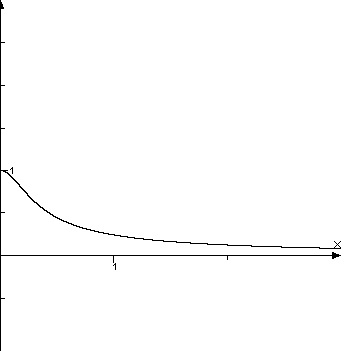
\includegraphics[width=0.5\textwidth]{amplitude.jpg}
					\footnotetext{Amplitudenverhältnis $\frac{x_0}{x_{0,ERR}}$ mit wachsender Dämpfung}
				\end{minipage}
				\begin{minipage}[t]{0.5\textwidth}
					\includegraphics[width=0.5\textwidth]{Phasenlage.jpg}
					\footnotetext{Phasenlage $\phi$ mit wachsender Dämpfung}
				\end{minipage}
			\end{figure}}
	\end{enumerate}
	
	
	
\end{document}